\documentclass[10pt,conference]{IEEEtran}

\usepackage[utf8]{inputenc}
\usepackage{cite}
\usepackage{hyperref}
\usepackage{graphicx}	% For figure environment

\begin{document}
\title{Characterization of turbulent flows in tokamaks}

\author{
  Julien Hu, Matthieu Masouyé and Sébastien Ollquist\\
  \textit{Department of Computer Science, EPFL, Switzerland}
}

\maketitle
\thispagestyle{plain}
\pagestyle{plain}

\begin{abstract}
    The goal of this project is to use machine learning to analyze GPI measures and estimate the Z-axis velocity of the structures.\par 
    To perform this task, we have implemented a convolutional neural network (CNN) to predict the speed of the gaz, on a synthetic dataset we generated ourselves and real data provided to us by the lab.\par
    We have tuned some hyperparameters to optimize the models and obtain the best results. We were able to successfully train and optimize a CNN for each dataset, and overall we were able to have good estimation of the speeds on the real data. 
\end{abstract}

\section{Introduction}
A tokamak is a device which uses a powerful magnetic field to confine hot plasma in the shape of a torus\cite{wikipediatokamak} (See Fig. \ref{figure:geometrytokamak}). At the edges of this field, it separates from the flow in a turbulent fashion. These turbulences might create blobs of plasma, that can be ejected at high speed.\par 
The technique used to study these turbulences is called Gas Puff Imaging (GPI). It generally consists of injecting a puff of neutral gas in this region, which will be excited by the plasma. This will create light emission, that are then collected tangentially to the magnetic field lines, allowing imaging of the turbulent structures.(See Fig. \ref{figure:gpiimage})\par

\begin{figure}[!b]
  \centering
  \begin{minipage}[b]{0.2\textwidth}
    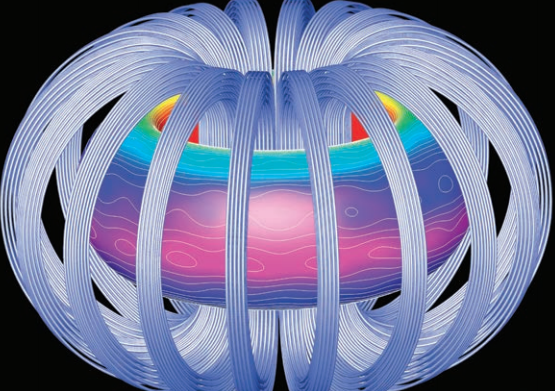
\includegraphics[width=\textwidth]{images/tokamak.png}
    \caption{Geometry of a tokamak\cite{tokamak}, which has the shape of a torus.}
    \label{figure:geometrytokamak}
  \end{minipage}
  \hfill
  \begin{minipage}[b]{0.18\textwidth}
    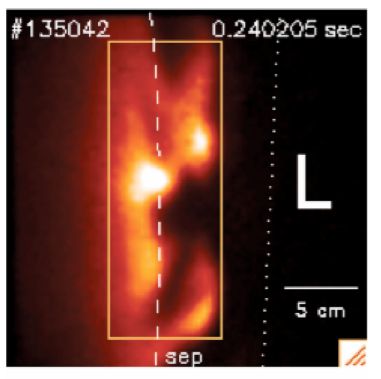
\includegraphics[width=\textwidth]{images/blob.PNG}
    \caption{GPI images from the tokamak, we can see the gaz excited by the plasma, and the white dashed line is the peripheral region of the plasma.\cite{zweben}}
    \label{figure:gpiimage}
  \end{minipage}
\end{figure}


GPI analysis is an ongoing task, and can yield important results. The Swiss Plasma Center lab at EPFL was interested in the new possibilities machine learning could bring, and together we worked to test how well a neural network could analyze these images.\par
 

 
The primary objective was to measure the $z$-axis velocities of the moving, turbulent structures captured by GPI. We have decided to opt for a convolutional neural network working on sequences of frames, as it is a good approach for complex tasks and convenient for image sequence analysis and velocity estimation \cite{velocitycnn}.



\section{Data and preprocessing}

\subsection{Real Data Description}
The labeled data was given to us from the lab in 9 pickle files, inside which there are the following sets:
\begin{enumerate}
  \item \texttt{shot} the shot number.
  \item \texttt{t\_window} an array of timestamps at which the frames were measured, in seconds
  \item \texttt{brt\_arr} a 3D-array (of 12x10x$l$ where $l$ is the length of \texttt{t\_window}) of G.P.I. measures, corresponding to the brightness of each 12 by 10 frames, measured in $mW/cm^2/ster$
  \item \texttt{r\_arr} the array of $r$-coordinate of each view, in meters.
  \item \texttt{z\_arr} the similar array of $z$-coordinate of each view, also in meters.
  \item \texttt{vz\_from\_wk} the vertical speed for each column of data, in $km/s$.
  \item \texttt{vz\_err\_from\_wk} the error margin in the estimation of vz
  \item \texttt{col\_r} the average $r$-coordinate of each column.
\end{enumerate}
Due to the measurement method, four specific "pixels" of \texttt{brt\_arr} are set to NaN permanently. The \texttt{r\_arr} and \texttt{z\_arr} describe the exact position of each pixel of \texttt{brt\_arr} in a 2d space, as they are not perfectly spaced. \texttt{vz\_from\_wk} will constitute the labels for the algorithm.\par
Importantly, there are 13 values in \texttt{vz\_from\_wk}, \texttt{vz\_err\_from\_wk} and \texttt{col\_r} while there are only 12 columns per frames: this is because the shear layer we want to calculate is inside one of the columns, which means this column will have flows going both ways. Thus, this column will have two speeds associated to it. \par
It wasn't possible for the lab to provide good estimates of these two speeds in all datasets, so the 13th column is set to NaN if there isn't an accurate estimation. We had to ignore these sets as that would have meant changing our approach too much; those concerned 3 out of the 9 different files.
Finally, the direction of the plasma relative to the shear layer is consistent: the left side always has plasma going down (i.e. negative values), while the right side always going up (i.e. positive values). \par
In total, we have access to 278 datapoints with the provided datasets.

\subsection{Synthetic Data Description}
We have decided to generate artificial data mainly because it would give us a controlled environment with no noise or imprecision in the labels, and also because it would make for a clearer model to train and analyze.\par
We have decided to generate the data in the following way: we draw a large canvas (480x480), and spawn gaussian arrays of varying random small sizes ( 264 arrays of 100 to 260 pixels) in random places. A ratio of these arrays are also set to negative values (around 33\%). To draw a frame, all the arrays are summed in the canvas, and values are limited to between 0 and 255 to stay in an 8 bit grayscale. Then, a smaller window at the center is taken and downsampled until it reaches the final size of 10x12, same as the real data.\par
At creation, these arrays are assigned a vertical speed given their horizontal coordinate by an hyperbolic tangent, with several settings to tweak its behaviour. To update their position at each iteration, the speed is simply added to their position. To get the labels, we can simply average this speed function over each column of the final window.\par
Everytime the script is run, it will generate a new folder inside \texttt{data/}, where the final frames will be put, with the labels, and various other information for debuging and for reproducibility purposes (like a speedplot or a list of settings).
At the beginning of the script there is a list of variables used as settings to tweak the behaviour of the generated dataset.
 
\begin{figure}
  \centering
  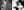
\includegraphics[scale=5]{images/comparison.png}
  \caption{Real image on the left, synthetic image on the right}
\label{comparison}
\end{figure}
 
This method gets reasonably close to how the real data looks like. You can see a side-to-side comparison in Fig. \ref{comparison}. In the precedent description, we have overseen a few simplifications in the behaviour of the synthetic dataset. For instance, the shear layer is always vertical but the real data's shear layer is slightly curved. Another important distinction is that the speed of the structures doesn't only go alongside the $z$-axis in the plasma. Simulating these aspects has been judged too complex for the stage of this project. Overall, the lab seemed satisfied with these synthetic datas.\par
To summarize, we have generated a total of 60 datapoints of 2000 frames each. We wanted to generate more, but we were limited by the computational power of our personal computers.
 


\subsection{Data Manipulation and Preprocessing}
We have implemented two different data loaders, that are used to organize and load real or synthetic data into the CNN.\par
Both data loaders organize the frames into 2000-frames datapoints (10x12x2000 values), and shuffle these datapoints using a fixed seed to homogenize the different scenarios. These datapoints are separated into 3 datasets: training, validation and testing sets, with default ratios of 64\%, 16\% and 20\% respectively. They will be used in the training and valudation phases, with testing only being used to evaluate our best model at the end.\par
The last transformation these datapoints need is to be converted from a 1-channel greyscale to 3-channel, to be compatible with the architectures we used. This was done simply by duplicating the single channel across the two others; this shouldn't pose any problem, because the model shouldn't depend on specific colors.\par
The differences between the two data loaders are where and how they fetch the frames, as they are stored in a different way on disk. Moreover, the dataloader working on real data has to rescale the values of the array to be 8-bit greyscale images instead of raw brightness measures. This isn't a problem for the synthetic dataloader as the synthetic data was already generated in a convenient way.

Due to time constraints, we could only use part of all the sets for the real data, that is, \texttt{t\_window}, \texttt{r\_arr}, \texttt{z\_arr} and \texttt{vz\_err\_from\_wk} were not taken into consideration for our algorithm.\par
Finally, the reason we chose to work with inputs of 2000 images is that on one side more images were pushing the limits of our computers in terms of time and memory. On the other, the lab estimated that an entire structure would take approximately 18'000 frames to cross the image completely, so 2'000 frames should mean it moves at least one pixel, as the images have a height of 10 pixels.\par


\section{Model training}
 
\subsection{The CNN architectures}
To perform our regression task, we have decided to work on the architectures defined for video classification in PyTorch, for simplicity and efficiency. We trust the architectures have already been optimized and tested,. It is hence easier and safer to use them rather than develop our own network. The architectures considered were: \textit{ResNet 3D}, \textit{ResNet Mixed Convolution} and \textit{ResNet (2+1)D} \cite{resnets}. ResNet is a classic neural network that helps solving computer vision tasks \cite{hara3dcnns}. As we have to analyze a sequence of images, this architecture is appropriate for our problem.\par
These networks consist of multiple processing layers that perform different operations to process the input, extract and recognise its key features (measurable property or characteristic), but also predict the desired outputs. These layers are:
\begin{itemize}
  \item The convolutional layer, in which features from input images or feature maps are extracted by applying filters.
  \item The pooling layer, that is similar to the convolutional layer, but performs a specific function, such as taking the maximum or average value in a region, to reduce the complexity and amount of computation of the network 
  \item The fully connected layer, where the network regroups all information from the final feature maps, and generates the output.
\end{itemize}

The main difference between the three architectures lies in the convolutional layers, where filters are applied distinctively:
\begin{itemize}
  \item ResNet 3D performs a 3D convolution, the 3D filters are convolved both over time and space dimensions.
  \item ResNet Mixed Convolution starts with 3D convolution, then in later layers, uses 2D convolution, as at higher level of abstraction, motion or temporal modeling may not be necessary.
  \item ResNet (2+1)D seperates the 3D convolution into two steps, a 2D convolution in the space dimension followed by a 1D convolution in time, to reduce the computation cost \cite{spacetimeconv}.
\end{itemize}

\subsection{The training procedure}
We start training it on the synthetic data so that we can get a good impression of how well it performs. We then train it on the real data.\par 
The training loop consists of two main phases: the training phase, where the model is first trained from the training set. The model learns how to recognize the key features, and will update its weights (learnable parameters) with its performance
on the dataset. \par 
Then, during the validation phase, the model simply predicts the output for the validation set, and computes the loss. This part is to give an estimation how good the model performs at each iteration, to detect any signs of overfitting. \par
Each step is repeated for 30 epochs. The last validation results are used to compare different instances of the model and choose the best hyperparameters. After optimizing and selecting the best performing model, it is then tested on the testing set, which contains data the model has never been executed with. The testing phase is only to provide us with an evaluation of the final model.



\subsection{Finding the correct architecture}
To find the most suitable model for our task, we have decided to train and evaluate it with our synthetic dataset. We see from the last validation results from table \ref{table:comparisonLoss}, that ResNet 3D offers the best results. Moreover, while training the models afterwards on the real dataset, our computers were unable to handle the ResNet MixedConv and ResNet 2+1D, as the memory load is too heavy with some set of hyperparameters, and would restrain us for optimization. We therefore selected and optimized ResNet 3D. 

\begin{table}[h!]
\centering
 \begin{tabular}{|c | c |} 
 \hline
    Architecture & Validation loss \\  
 \hline\hline
    ResNet 3D & 1.181\\ 
 \hline
    ResNet MixedConv & 3.792\\
 \hline
    ResNet 2+1D & 3.284\\
 \hline
\end{tabular}
\caption{Last validation results for the architectures after 30 epochs.}
\label{table:comparisonLoss}
\end{table}

After choosing the architecture to work on, we also needed to get the optimal hyperparameters. The hyperparameters we chose to improve the model with were:
\begin{itemize}
  \item The learning rate \textit{lr}, which describes how much should it update itself based on the error. Choosing a learning rate that is too high can cause the model to converge too quickly to a sub-optimal solution or overfit the training data, while a too low learning rate results in a long training process, or can even cause the model to be stuck.
  \item \textit{batch\_size}, which defines the number of samples that will be trained at the same time, and affects how the gradient is calculated when correcting the weights. In short, bigger batches means the gradient should fluctuate less and be more accurate, at the expense of memory required. But it doesn't necessarily means a better model, as a noisier gradient might lead to a more robust model.
\end{itemize}
 
%The smaller the batch the less accurate the estimate of the gradient will be. In the figure below, you can see that the direction of the mini-batch gradient (green color) fluctuates much more in comparison to the direction of the full batch gradient (blue color). 
The loss function used to evaluate the model is the MSE (Mean Square Error) loss function, as it is the most commonly used function for regression tasks. As for the optimizer, we decided to choose SGD. We tested with Adam, but the model struggled to converge, and resulted in worse losses. We have also used a scheduler, which causes the learning rate to decrease after some epochs, so that the model converges safely. The $\gamma$ has been set to 0.1 and the step\_size to 10, as we didn't have time to optimize them. The seeds are the same for all the models.


%Possible que la validation loss soit meilleure au début du training qu'à la fin, mais sur le graph, on peut voir que la training loss est quand meme tres haute, et que la validation est instable au début et donc pas représentatif d'une bonne performance du modèle.
\section{Results}

\begin{table}[h]
    \centering
    \begin{tabular}{|c || c | c | c | c | c | c| c | c |} 
        \hline
           & 0.01 & 0.02 & 0.03 & 0.04 & 0.05 & 0.06 \\  
        \hline\hline
        2  & 2.81 & 1.50 & 2.54 &      &      &\\ 
        \hline
        4  & 2.74 & 1.25 & 1.05 & 1.59 &      &\\
        \hline
        8  &      & 3.77 & 1.16 & 1.02 & 2.48 &\\
        \hline
        16 &      & 5.76 & 4.02 & 3.97 & 3.12 & 4.00\\
        \hline
    \end{tabular}
    \caption{Batch size (column) vs learning rate (rows) on synthetic data}
\label{table:syntheticDataResults}
\end{table}
\begin{table}[h]
    \centering
     \begin{tabular}{|c || c | c | c | c | c | c| } 
     \hline
        & 0.001& 0.005 & 0.01  & 0.02 & 0.03 & 0.04 \\  
     \hline\hline
     2  &      &       & 7.653 & 2.394& 1.863& 3.089 \\ 
     \hline
     4  &      &       & 0.377 & 0.268& 0.256& 0.359\\
     \hline
     8  & 0.213&  0.093& 0.111 & 0.133& 0.247&  \\
     \hline
     16 & 0.153&  0.116& 0.126 & 0.375&      &  \\
     \hline
    \end{tabular}
    \caption{Batch size (column) vs learning rate (rows) on the real data}
\label{table:realDataResults}
\end{table}


The results of our model on the synthetic data can be found in table \ref{table:syntheticDataResults}, and the ones on real data in table \ref{table:realDataResults}. The losses and models are from the last epoch of the algorithm. Note that not all cases have been tested. In fact, we stopped increasing the learning rate when the loss got worse. As for the batch size, we were again limited by our computing power, and 16 was the most we could run with.\par
It is also important to note that the losses of both datasets are not directly comparable; indeed, the synthetic dataset and real dataset do not use the same scale for measuring speed in their labels.\par

\subsection{Synthetic Dataset}
The losses throughout the epochs are a bit unstable: they often oscillate while converging, and only calm down after the decrease of the learning rate, at the tenth epoch. A good example of this is in Fig \ref{figure:oscillations}. We think this is due to both the fact that we don't have that many datapoints, and the fact that the different datasets have too many variations between them; the model has trouble learning it all. \par

\begin{figure}[h]
  \centering
  \begin{minipage}[h]{0.23\textwidth}
    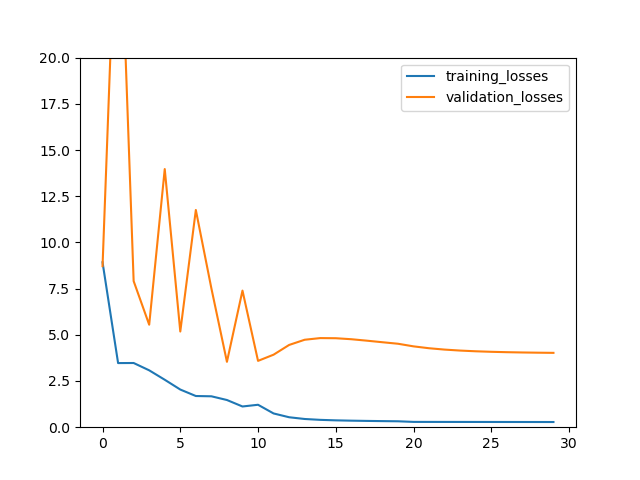
\includegraphics[width=\textwidth]{images/oscillations.png}
    \caption{Training and validation losses on synthetic dataset with learning rate 0.06 and batch size 16, we observe some oscillation until epoch 10.}
    \label{figure:oscillations}
  \end{minipage}
  \hfill
  \begin{minipage}[h]{0.23\textwidth}
    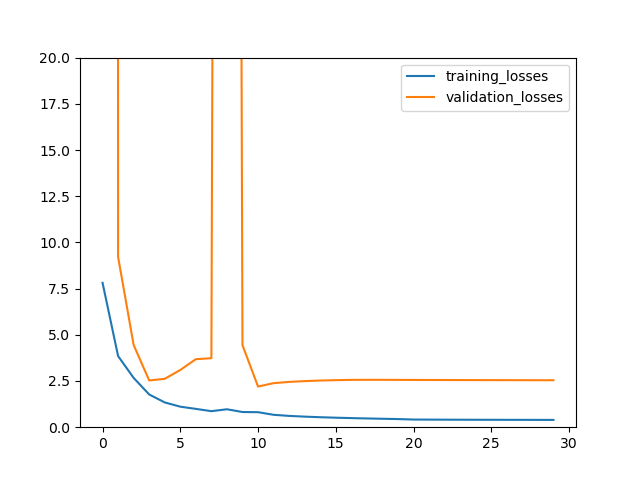
\includegraphics[width=\textwidth]{images/example_high_lr.png}
    \caption{Training and validation losses on synthetic dataset with learning rate 0.03 and batch size 2, a learning rate too high means the gradient is too big, and the model has trouble finding the optimal parameters}
    \label{figure:highlr}
  \end{minipage}
\end{figure}

Another sign that our synthetic dataset is too complex for the amount of datapoints is that the model does worse with a high batch size. Higher batch sizes tend to degrade a model's ability to generalize, and a batch size of 16 was close to half the datapoints available for training.
\subsection{Real Dataset}
The real dataset exhibits a strange behavior at higher batch sizes: the validation loss starts going under the training loss, as it can be seen in Fig \ref{figure:validation}. We unfortunately do not have a definite explanation, but our theory is that since there are only 6 different labels for all the real dataset, it can optimize all of them at once (on average) when the batch size is more than 6. It will find the gradient that maximizes all the different labels instead of only a few at a time. This means it will be more robust, and achieve a better validation, but it will have a harder time fitting all the training examples at once in comparison. This is supported by the fact that the validation loss is instantly under the train loss, whilst the train loss takes a while to decrease. The gradient however goes in a very robust direction from the begining of the training.\par
Another possibility is that the validation set has easier examples than the training set, but it is not consistent with the batch size. It should happen on all batch sizes.\par
Finally it might be an oversight in the loss calculation on our part. Perhaps we have forgotten a factor somewhere. This is not really consistent with the rest of the results, and the quality of the predictions, an example of which is in Fig. \ref{figure:predictions}.

\begin{figure}[h]
  \centering
  \begin{minipage}[h]{0.23\textwidth}
    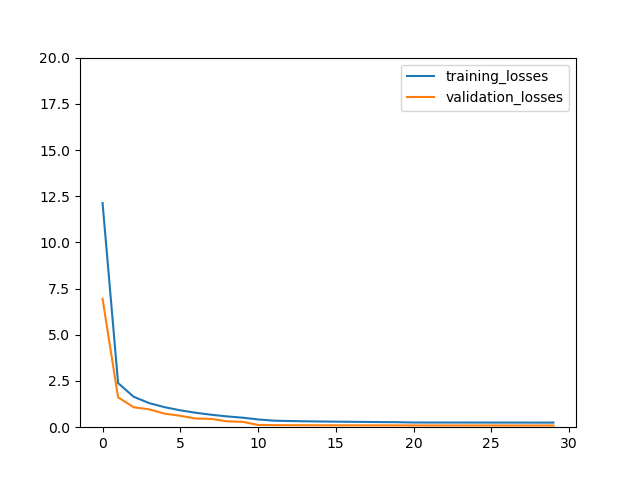
\includegraphics[width=\textwidth]{images/validation.png}
    \caption{Training and validation losses with learning rate 0.005 and batch size 8, unusual behavior from validation loss relative to train loss.}
    \label{figure:validation}
  \end{minipage}
  \hfill
  \begin{minipage}[h]{0.23\textwidth}
    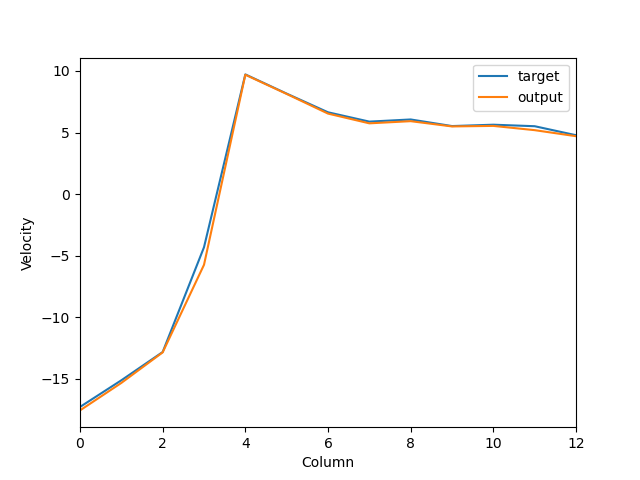
\includegraphics[width=\textwidth]{images/predictions.png}
    \caption{Example prediction and label with learning rate 0.005 and batch size 8 on the validation set.}
    \label{figure:predictions}
  \end{minipage}
\end{figure}


\section{Conclusion}
We have during this project implemented a method to automatically detect particle velocities when analyzing a sequence of images, using a CNN. We expected to train the CNN as we would do for a human, all this in order for it to learn quickly and efficiently.\par
We started by generating synthetic data to train the model on it before passing it the real data provided by the lab. Then, we had to select a model to train. We preferred using an already performant model proposed by PyTorch instead of creating all one by ourselves. This saved us much time and permitted us to directly train it for the kind of data we were using. The training on the synthetic data permitted us to estimate some good parameters to use for the model such as the learning rate and the batch size. We have in the end found pretty optimal parameters to use, which were close to 0.004 for the learning rate and a batch size of 8. Our results were quite encouraging, given the fact that the model can learn well and gives us small validation and training losses.\par
Due to time constraints, we could not find the optimum parameters, nor train on a different model but we could possibly in a future project, find other models to train, choose the perfect hyperparameters and eventually extend the role of the CNN to other kinds of identification on the given sequence of images.

\bibliographystyle{IEEEtran}
\bibliography{project2}

\end{document}